\chapter{Part C: Asset}
Developer: Yann Renoux

\noindent Validator: Joseph Perez


%DEVELOPER WRITES THIS PART --->

\section{Requirements}

\par This is an underlying asset class. It has a currency, a spot price level and a dividend
 schedule or a fixed dividend rate. It also possesses a yield curve, supposingly in his currency of denomination, which purpose is to discount future flows. We have made the choice not to use it as a member for the other classes, but it bears all the necessary information. It could be used as to provide a dividend growing rate for Black Scholes object for example.

Hence the choice has been made not to use an asset with a volatility surface that would simulate itself forward prices, as indeed it would be a single simulated price, and in expectation, the volatility does not enter into account.

The only purpose of this object is to be able to be added in the portfolio to hedge options on the book.

\section{Design }

\par Obviously a stock is a delta one security, the interesting thing is the benefit of carry with the dividends versus its cost of carry against the money we would get while depositing the money at the current market rate.

The other thing is that usually, with no inside information on the company, one cannot know for sure the future dividends that will be paid. Thus we decided to add the fixed dividend rate, which in practise would be an econometrically estimated parameter, but a very commonly used input in pricing, such as in Black-Scholes for instance.

The well-known formula for pricing a stock with dividends is:
\[
P_t=\sum_{i=1}^\infty Dividend_{t+i}\times DiscountFactor(t,t+i)
\]

Hence the forward price:
\[
F(t,T)=P_T=\sum_{i=1}^\infty Dividend_{T+i}\times DiscountFactor(t,T+i)
\]
In practise it would be the current price minus the known future dividends up to the date $T$. This entails and reflects the drop in price that a stock sustains when a dividend is paid: it theoretically decreases its current price by the exact amount that has been paid. On the contrary, with a fixed dividend rate $q$, the forward price is $F(t,T)=P_t e^{-q(T-t)}$. The following graph reflects this noticed fact.
\begin{figure}
\begin{center}
        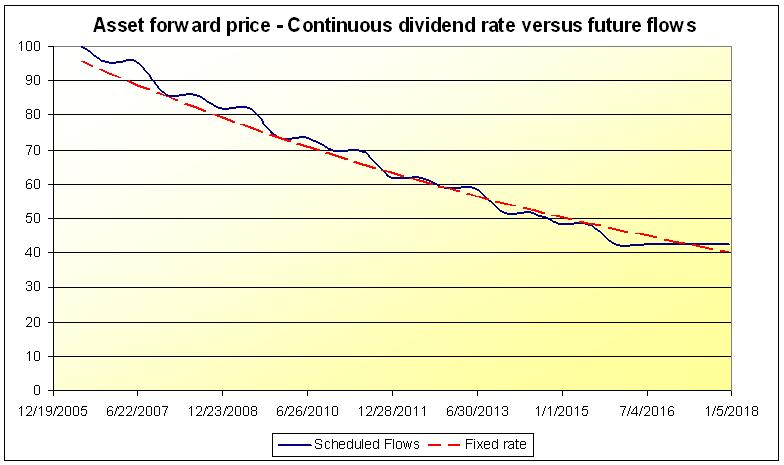
\includegraphics[width=12cm]{assetFWD.jpg}
        \caption{Asset forward price - comparison of a fixed continuous rate versus a dividend schedule}
\end{center}
\end{figure}

The continuous rate has been taken equal to $7.5\%$, while for the purpose of demonstration, the dividend schedule in the other case is up to 10 years, with $5\%$ the even years, and $10\%$ the odd years. The first noticeable fact is the sudden drop when the dividend is paid. This is not on an accrual basis as the bonds! On the other hand, the graph goes beyond the 10 years, and we remark that by then the forward price of the dividend scheduled asset remains constant, which is in agreement with the formula. Last note that the apparently increasing forward price is not the reality, it is just due to smoothing in Excel graph -- look at the output file produced by the test menu to check it.


\section{Approach}

\par The dividend schedule is a valarray of flowSchedule, a class with a date, an amount in percent, and a business day convention for the payment date. Indeed, if the payment date does not fall on a working day, the accrued interest calculation can differ depending on the convention.

An asset then has the mentionned members, should the user specify in the constructor the type of dividend, fix rate or scheduled. All the methods check this before pricing.


\section{Methods}

\par The forward price is using the formulas mentionned above, and the class has a getDelta function so that the portfolio class can know that holding an asset is delta one.

\par The getPrice method has been made virtual so that if later we want to inherit from this, we can do it.

\section{Unit tests}

\par We have tested several dividend rates, and schedules, checking that the forward drops on the payment date by the expected amount. The output file for the 10 year dividends illustrates well what we did.

\section{Performance}

\par This class being rather simple, nothing huge can be done to make it quicker. And if so, this was not at all the most important object to improve. See the mainasset in the test directory for more details.


\section{Validation}
No particular validation test were needed for this simple class, we just had to check that code had no bug and formula for forward price was correct.

